% Figura cuerpo B2: el mismo aparato explica el ciclo y el crecimiento; solo cambian tamaño y persistencia
\documentclass[tikz,border=3pt]{standalone}
\usepackage[T1]{fontenc}
\usepackage[utf8]{inputenc}
\usepackage{amsmath}
\usetikzlibrary{arrows.meta,calc,positioning}
\begin{document}
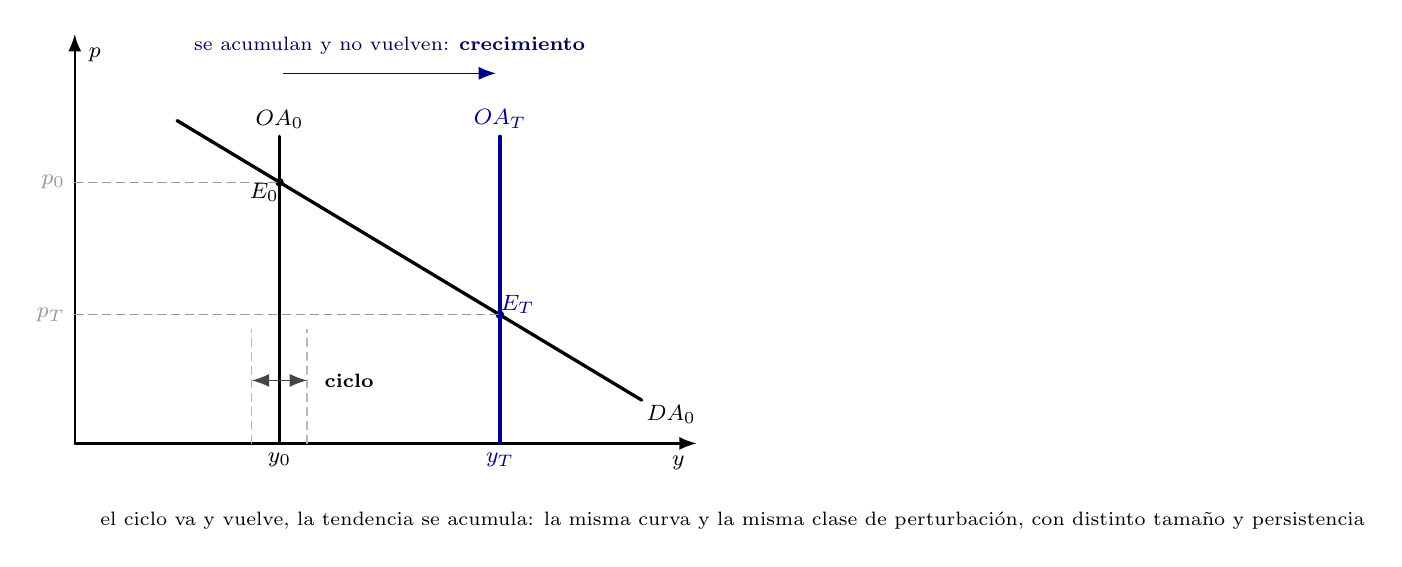
\begin{tikzpicture}[>={Latex[length=2.2mm]}, line cap=round, font=\footnotesize,
  eje/.style={->, thick},
  curva/.style={very thick},
  nueva/.style={very thick, blue!55!black},
  guia/.style={densely dashed, gray!80},
  tenue/.style={densely dashed, gray!55},
  pto/.style={circle, fill=black, inner sep=1.1pt}]
  \draw[eje] (0,0) -- (7.9,0) node[below left=1pt]{$y$};
  \draw[eje] (0,0) -- (0,5.2) node[below right=2pt]{$p$};
  % Demanda
  \draw[curva] (1.3,4.1) -- (7.2,0.55) node[below right=-3pt]{$DA_0$};
  % Ofertas verticales: la de partida y la que deja la acumulación de perturbaciones persistentes
  \draw[curva] (2.6,0) -- (2.6,3.9) node[above=-1pt]{$OA_0$};
  \draw[nueva] (5.4,0) -- (5.4,3.9) node[above=-1pt]{$OA_T$};
  % Banda del ciclo alrededor de la oferta de partida
  \draw[tenue] (2.25,0) -- (2.25,1.45);
  \draw[tenue] (2.95,0) -- (2.95,1.45);
  \draw[<->, gray!55!black] (2.25,0.8) -- (2.95,0.8);
  \node[anchor=west, font=\scriptsize] at (3.05,0.8) {\textbf{ciclo}};
  % Deriva de la tendencia
  \draw[->, blue!55!black] (2.65,4.7) -- (5.35,4.7);
  \node[anchor=south, font=\scriptsize, align=center, text=blue!35!black] at (4.0,4.82)
    {se acumulan y no vuelven: \textbf{crecimiento}};
  % Equilibrios
  \node[pto] (E0) at (2.6,3.318) {};
  \node[below left=-3pt of E0, inner sep=1pt] {$E_0$};
  \node[pto, fill=blue!55!black] (ET) at (5.4,1.633) {};
  \node[above right=-3pt of ET, inner sep=1pt, blue!55!black] {$E_T$};
  \draw[guia] (0,3.318) node[left]{$p_0$} -- (2.6,3.318);
  \draw[guia] (0,1.633) node[left]{$p_T$} -- (5.4,1.633);
  \node[below] at (2.6,0) {$y_0$};
  \node[below, text=blue!55!black] at (5.4,0) {$y_T$};
  \node[align=left, anchor=north west, font=\scriptsize] at (0.2,-0.75)
    {el ciclo va y vuelve, la tendencia se acumula: la misma curva y la misma clase de perturbación, con distinto tamaño y persistencia};
\end{tikzpicture}
\end{document}
